\documentclass[12pt,-letter paper]{article}                       
\usepackage{siunitx}                                              
\usepackage{setspace}
\usepackage{gensymb}                                              
\usepackage{xcolor}                                               
\usepackage{caption}
%\usepackage{subcaption}
\doublespacing                                                   
\singlespacing                                                    
\usepackage[none]{hyphenat}
\usepackage{amssymb}
\usepackage{relsize}
\usepackage[cmex10]{amsmath}
\usepackage{mathtools}
\usepackage{amsmath}                                              
\usepackage{commath}                                              
\usepackage{amsthm}
\interdisplaylinepenalty=2500
%\savesymbol{iint}
\usepackage{txfonts}                                              
%\restoresymbol{TXF}{iint}                                        
\usepackage{wasysym}                                              
\usepackage{amsthm}
\usepackage{mathrsfs}                                             
\usepackage{txfonts}                                              
\let\vec\mathbf{}
\usepackage{stfloats}
\usepackage{float}
\usepackage{cite}
\usepackage{cases}                                                
\usepackage{subfig}                                               
%\usepackage{xtab}
\usepackage{longtable}
\usepackage{multirow}
%\usepackage{algorithm}
\usepackage{amssymb}
%\usepackage{algpseudocode}
\usepackage{enumitem}
\usepackage{mathtools}
%\usepackage{eenrc}
%\usepackage[framemethod=tikz]{mdframed}                          
\usepackage{listings}                                             
%\usepackage{listings}
\usepackage[latin1]{inputenc}
%%\usepackage{color}{
%%\usepackage{lscape}
\usepackage{textcomp}
\usepackage{titling}
\usepackage{hyperref}
%\usepackage{fulbigskip}
\usepackage{tikz}
\usepackage{graphicx}                                             
\lstset{
  frame=single,
  breaklines=true
}
\let\vec\mathbf{}
\usepackage{enumitem}                                             
\usepackage{graphicx}                                             
\usepackage{siunitx}
\let\vec\mathbf{}                                                
\usepackage{enumitem}
\usepackage{graphicx}
\usepackage{enumitem}
\usepackage{tfrupee}
\usepackage{amsmath}
\usepackage{amssymb}
\usepackage{mwe} % for blindtext and example-image-a in example
\usepackage{wrapfig}
\usepackage{enumitem}
\providecommand{\qfunc}[1]{\ensuremath{Q\left(#1\right)}}
\providecommand{\sbrak}[1]{\ensuremath{{}\left[#1\right]}}
\providecommand{\brak}[1]{\ensuremath{\left(#1\right)}}
\providecommand{\lbrak}[1]{\ensuremath{\left(#1\right.}}
\providecommand{\rbrak}[1]{\ensuremath{\left.#1\right)}}
\providecommand{\cbrak}[1]{\ensuremath{\left\{#1\right\}}}
\providecommand{\lcbrak}[1]{\ensuremath{\left\{#1\right.}}
\providecommand{\rcbrak}[1]{\ensuremath{\left.#1\right\}}}
\begin{document}
\title{GEOMETRY - CBSE}
\author{TIRUMALA SAI NITHIN}
\date{Dec 2023}
\maketitle
\begin{enumerate}
\item The radius of a sphere (in cm) whose volume is $12\pi cm^3$, is
\begin{enumerate}
\item $3$
\item $3 \sqrt{3}$
\item $3^\frac{2}{3}$
\item $3^\frac{1}{3}$
\end{enumerate}
\item In \figref{fig:Fig-4.png}, the angle of elevation of the top of a tower from a point $C$ on the ground, which is $30m$ away from the foot of the tower, is $30\degree$. Find the height of the tower.      
\begin{figure}[H]
\centering
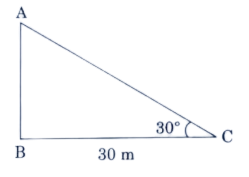
\includegraphics[width=\columnwidth]{Documents/Projects/Figures/Fig-4.png}
\caption{}      
\label{fig:Fig-4.png}
\end{figure}
\item A cone and a cylinder have the same radii but the height of the cone is $3$ times that of the cylinder. Find the ratio of their volumes.
\item In \figref{fig:Fig-8.png}, $ABCD$ is a parallelogram. A semicircle with centre $O$ and the diameter $AB$ has been drawn and it passes through $D$. If $AB=12cm$ and $OD \perp AB$, then find the area of the shaded region. (Use $\pi=3.14$)
\begin{figure}[H]
\centering
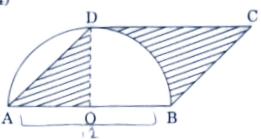
\includegraphics[width=\columnwidth]{Documents/Projects/Figures/Fig-8.png}
\caption{}
\label{fig:Fig-8.png}
\end{figure}
\item A statue $1.6m$ tall, stands on the top of a pedestal. From a point on the ground, the angle of elevation of the top of the statue is $60\degree$ and from the same point the angle of elevation of the top of the pedestal is $45\degree$. Find the height of the pedestal.(Use $\sqrt{3}=1.73$)
\item In a cylindrical vessel of radius $10 cm$, containing some water, $9000$ small spherical balls are dropped which are completely immersed in water which raises the water level. If each spherical ball is of radius $0.5 cm$, then find the rise in the level of water in the vessel.
\item If a line is drawn parallel to one side of a triangle to intersect the other two sides at distinct points, prove that the other two sides are divided in the same ratio.
\item If $\tan^{-1}\brak{\frac{y}{x}}=\log\sqrt{x^2+y^2}$, prove that $\frac{dy}{dx}=\frac{x+y}{x-y}$.
\item If $y=e^{a \cos^{-1}x}, -1<x<1$, then show that
\begin{align}	
	\brak{1-x^2}\frac{d^2y}{dx^2}-x\frac{dy}{dx}-a^2y=0
\end{align}
\end{enumerate}
\end{document}
